\documentclass[12pt]{article}
%\usepackage[margin=lin]{geometry}
\usepackage{amsmath,amsthm,amssymb,amsfonts}
\usepackage{graphicx}

\graphicspath{ {images/} }

\newtheorem*{problem}{Problem}

\theoremstyle{definition}
\newtheorem*{solution}{Solution}

\begin{document}

\title{AC Circuits Homework 2}
\author{Daniel Halmrast}
\maketitle

%--PROBLEM 1--%
\begin{problem}[1.a]
Consider an RLC circuit with source voltage $V_s = V_0 \sin(\omega t)$.
Determine the current $I = I_0 \sin(\omega t + \phi)$.
\end{problem}

\begin{solution}[1.a]
Our defining differential equation is
\[
	V_S = \frac{1}{C}Q(t) + R\frac{dQ}{dt} + L\frac{d^2Q}{dt^2}
\]
Or, in more familiar terms of $I$,
\[
	V_S = \frac{1}{C}\int_0^t Idt + RI + L\frac{dI}{dt}
\]

Substituting $I = I_0 \sin(\omega t + \phi)$ and $V_s = V_0 \sin(\omega t)$ we get
\[
\begin{aligned}
	V_0 \sin(\omega t) 
	& = \frac{1}{C}\int_0^t I_0 \sin(\omega t + \phi)dt + R I_0 \sin(\omega t + \phi)+ L\frac{d}{dt}I_0 \sin(\omega t + \phi)\\
\\
	& = I_0 \Big[ \frac{-1}{C\omega}\cos(\omega t + \phi) + R \sin(\omega t + \phi) + L\omega \cos(\omega t + \phi)\Big]
\end{aligned}
\]
Using sum of angles identites, we split the RHS into $\sin(\omega t)$ and $\cos(\omega t)$ parts.

\[
\begin{aligned}
	V_0 \sin(\omega t) 
	& = \Big[ I_0R\cos(\phi) + \big(\frac{I_0}{C\omega}-I_0L\omega\big)\sin(\phi) \Big]\sin(\omega t)\\
	& + \Big[ I_0R\sin(\phi) + \big(I_0L\omega-\frac{I_0}{C\omega}\big)\cos(\phi) \Big]\cos(\omega t)
\end{aligned}
\]

Equating the coefficients yields two equations.
\[
\begin{aligned}
V_0 & = I_0R\cos(\phi) + \big(\frac{I_0}{C\omega}-I_0L\omega\big)\sin(\phi)\\
0   & = I_0R\sin(\phi) + \big(I_0L\omega-\frac{I_0}{C\omega}\big)\cos(\phi)
\end{aligned}
\]

The second equation simplifies to
\[
R\sin(\phi) = \big(\frac{1}{C\omega}-L\omega\big)\cos(\phi)\\
\]
\begin{equation}
\boxed{\tan(\phi) = \frac{\frac{1}{C\omega}-L\omega}{R}}
\end{equation}
This immediately yields the following useful identities
\begin{equation}
\sin(\phi) = \frac{\frac{1}{C\omega}-L\omega}{\sqrt{R^2 + (\frac{1}{C\omega}-L\omega)^2}}
\end{equation}

\begin{equation}
\cos(\phi) = \frac{R}{\sqrt{R^2 + (\frac{1}{C\omega}-L\omega)^2}}
\end{equation}

Going back to the first coefficient equality, and using results 2 and 3, we see that
\[
\begin{aligned}
V_0 & = I_0R\cos(\phi) + \big(\frac{I_0}{C\omega}-I_0L\omega\big)\sin(\phi)\\
    & = I_0 \Big[ R\frac{R}{\sqrt{R^2 + (\frac{1}{C\omega}-L\omega)^2}} + \big(\frac{I_0}{C\omega}-I_0L\omega\big)\frac{\frac{1}{C\omega}-L\omega}{\sqrt{R^2 + (\frac{1}{C\omega}-L\omega)^2}}\Big]\\
    & = I_0 \Big[\frac{R^2 + \big(\frac{1}{C\omega}-L\omega\big)^2}{\sqrt{R^2 + (\frac{1}{C\omega}-L\omega)^2}}\Big]\\
\\
    & = I_0 \sqrt{R^2 + (\frac{1}{C\omega}-L\omega)^2}
\end{aligned}
\]
Therefore
\begin{equation}
\boxed{I_0 = \frac{V_0}{(R^2 + (\frac{1}{C\omega}-L\omega)^2)^{\frac{1}{2}}}}
\end{equation}

\end{solution}

%--PROBLEM 2--%
\setcounter{equation}{0}
\begin{problem}[1.b]
Graph $\phi(\omega)$.
\end{problem}

\begin{solution}[1.b]
$\phi$ is defined implicitly by

\begin{equation}
\tan(\phi)  = \frac{\frac{1}{C\omega}-L\omega}{R}
\end{equation}

Which we will explicitly write as

\begin{equation}
\phi(\omega) = \arctan\Big(\frac{\frac{1}{C\omega}-L\omega}{R}\Big)
\end{equation}

Clearly, as $\omega \to 0$, we have $\phi \to \arctan(\infty) = \frac{\pi}{2}$.
Also, when $\omega = \frac{1}{\sqrt{LC}}$, $\phi = 0$.
\\
A graph of $\phi(\omega)$ for $L = C = 1$ is shown.\\
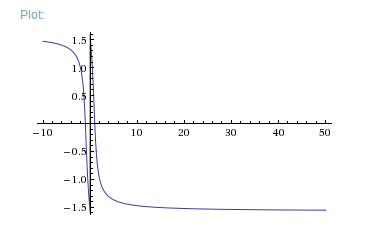
\includegraphics[scale=0.7]{RLC_total_phase}

\end{solution}

%--PROBLEM 3--%
\setcounter{equation}{0}
\begin{problem}[1.c]
Plot $V_{R_0}(\omega)$.
\end{problem}

\begin{solution}[1.c]

By the relation $V_R = IR$, $V_{R_0}$ is $RI_0$
Thus
\begin{equation}
V_{R_0}(\omega) = \frac{V_0R}{(R^2 + (\frac{1}{C\omega}-L\omega)^2)^{\frac{1}{2}}}
\end{equation}
It is easy to see that when $\omega \to 0$, $V_R \to 0$. 
Also, $V_R$ attains a maximum at the characteristic frequency $\omega = \frac{1}{\sqrt{LC}}$.\\

A graph of $V_{R_0}(\omega)$ for $V_0 = L = C = 1$ is shown.\\
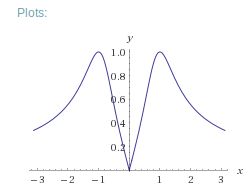
\includegraphics[scale=0.7]{RLC_res_voltage}

\end{solution}

%--PROBLEM 4--%
\setcounter{equation}{0}
\begin{problem}[1.d]
Solve for the voltage across the capacitor, using $V_C = \frac{Q(t)}{C}$
\end{problem}

\begin{solution}[1.d]

Rewriting $V_C$ in a more familiar form, we have
\[
\begin{aligned}
V_C & = \frac{1}{C}\int_0^t I dt\\
    & = \frac{1}{C}\int_0^t I_0 \sin(\omega t + \phi)dt
\end{aligned}
\]
Which yields
\[
V_C = \frac{-I_0}{C\omega}\cos(\omega t + \phi)
\]
With
\begin{equation}
I_0         = \frac{V_0}{(R^2 + (\frac{1}{C\omega}-L\omega)^2)^{\frac{1}{2}}}
\end{equation}
\begin{equation}
\tan(\phi)  = \frac{\frac{1}{C\omega}-L\omega}{R}
\end{equation}

The reader is now encouraged to recall the trigonometry identity relating $\sin$ and $\cos$
\[
\cos(x) = \sin(x + \frac{\pi}{2})
\]

Thus, $V_C$ can be expressed in terms of the $\sin$ function as 
\[
\begin{aligned}
V_C & = \frac{-I_0}{C\omega}\sin(\omega t + \phi + \frac{\pi}{2})\\
    & = \frac{I_0}{C\omega}\sin(\omega t + \phi - \frac{\pi}{2})
\end{aligned}
\]
\end{solution}
\end{document}

